\documentclass[10pt]{article}
\usepackage[a4paper,margin=2cm]{geometry}
\usepackage[brazilian]{babel}
\usepackage[utf8]{inputenc}
\usepackage[T1]{fontenc}
\linespread{1.3}
\parskip=12pt
\parindent=0pt
\usepackage{enumerate}
\usepackage{amsfonts}
\usepackage{amsmath}
\usepackage{amsfonts}
\usepackage{graphicx}

\begin{document}
	\begin{center}
		{\Large{\textbf{Lista 4 - Macroeconomia III 2017}}}\\
		\vspace{0.2cm}
		Alunos: Alexandre Machado e Raul Guarini\\
		Monitora: Kátia Alves
	\end{center}
	
\section*{Exercício 1}
A matriz F calculada é como abaixo:
\begin{center}
	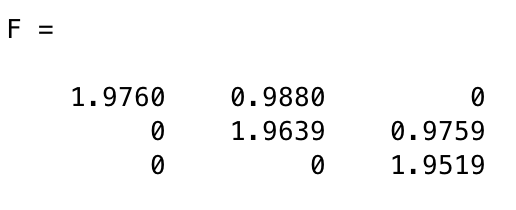
\includegraphics[scale = 0.7]{F}
\end{center}

O consumo ótimo esta derivado no código. A matriz F de autarquia é uma matriz de zeros, uma vez que nesse caso ninguém faz depósitos e, por definição, usa a tecnologia de estocagem de maneira individual.

O bem-esta ótimo foi calculado em -0.9761 e o de autarquia em -0.9762. Logo, os consumidores preferem de fato o arranjo bancário. Com relação ao bem-estar de corrida, este foi calculado como -1. Abaixo, o gráfico pedido:

\begin{center}
	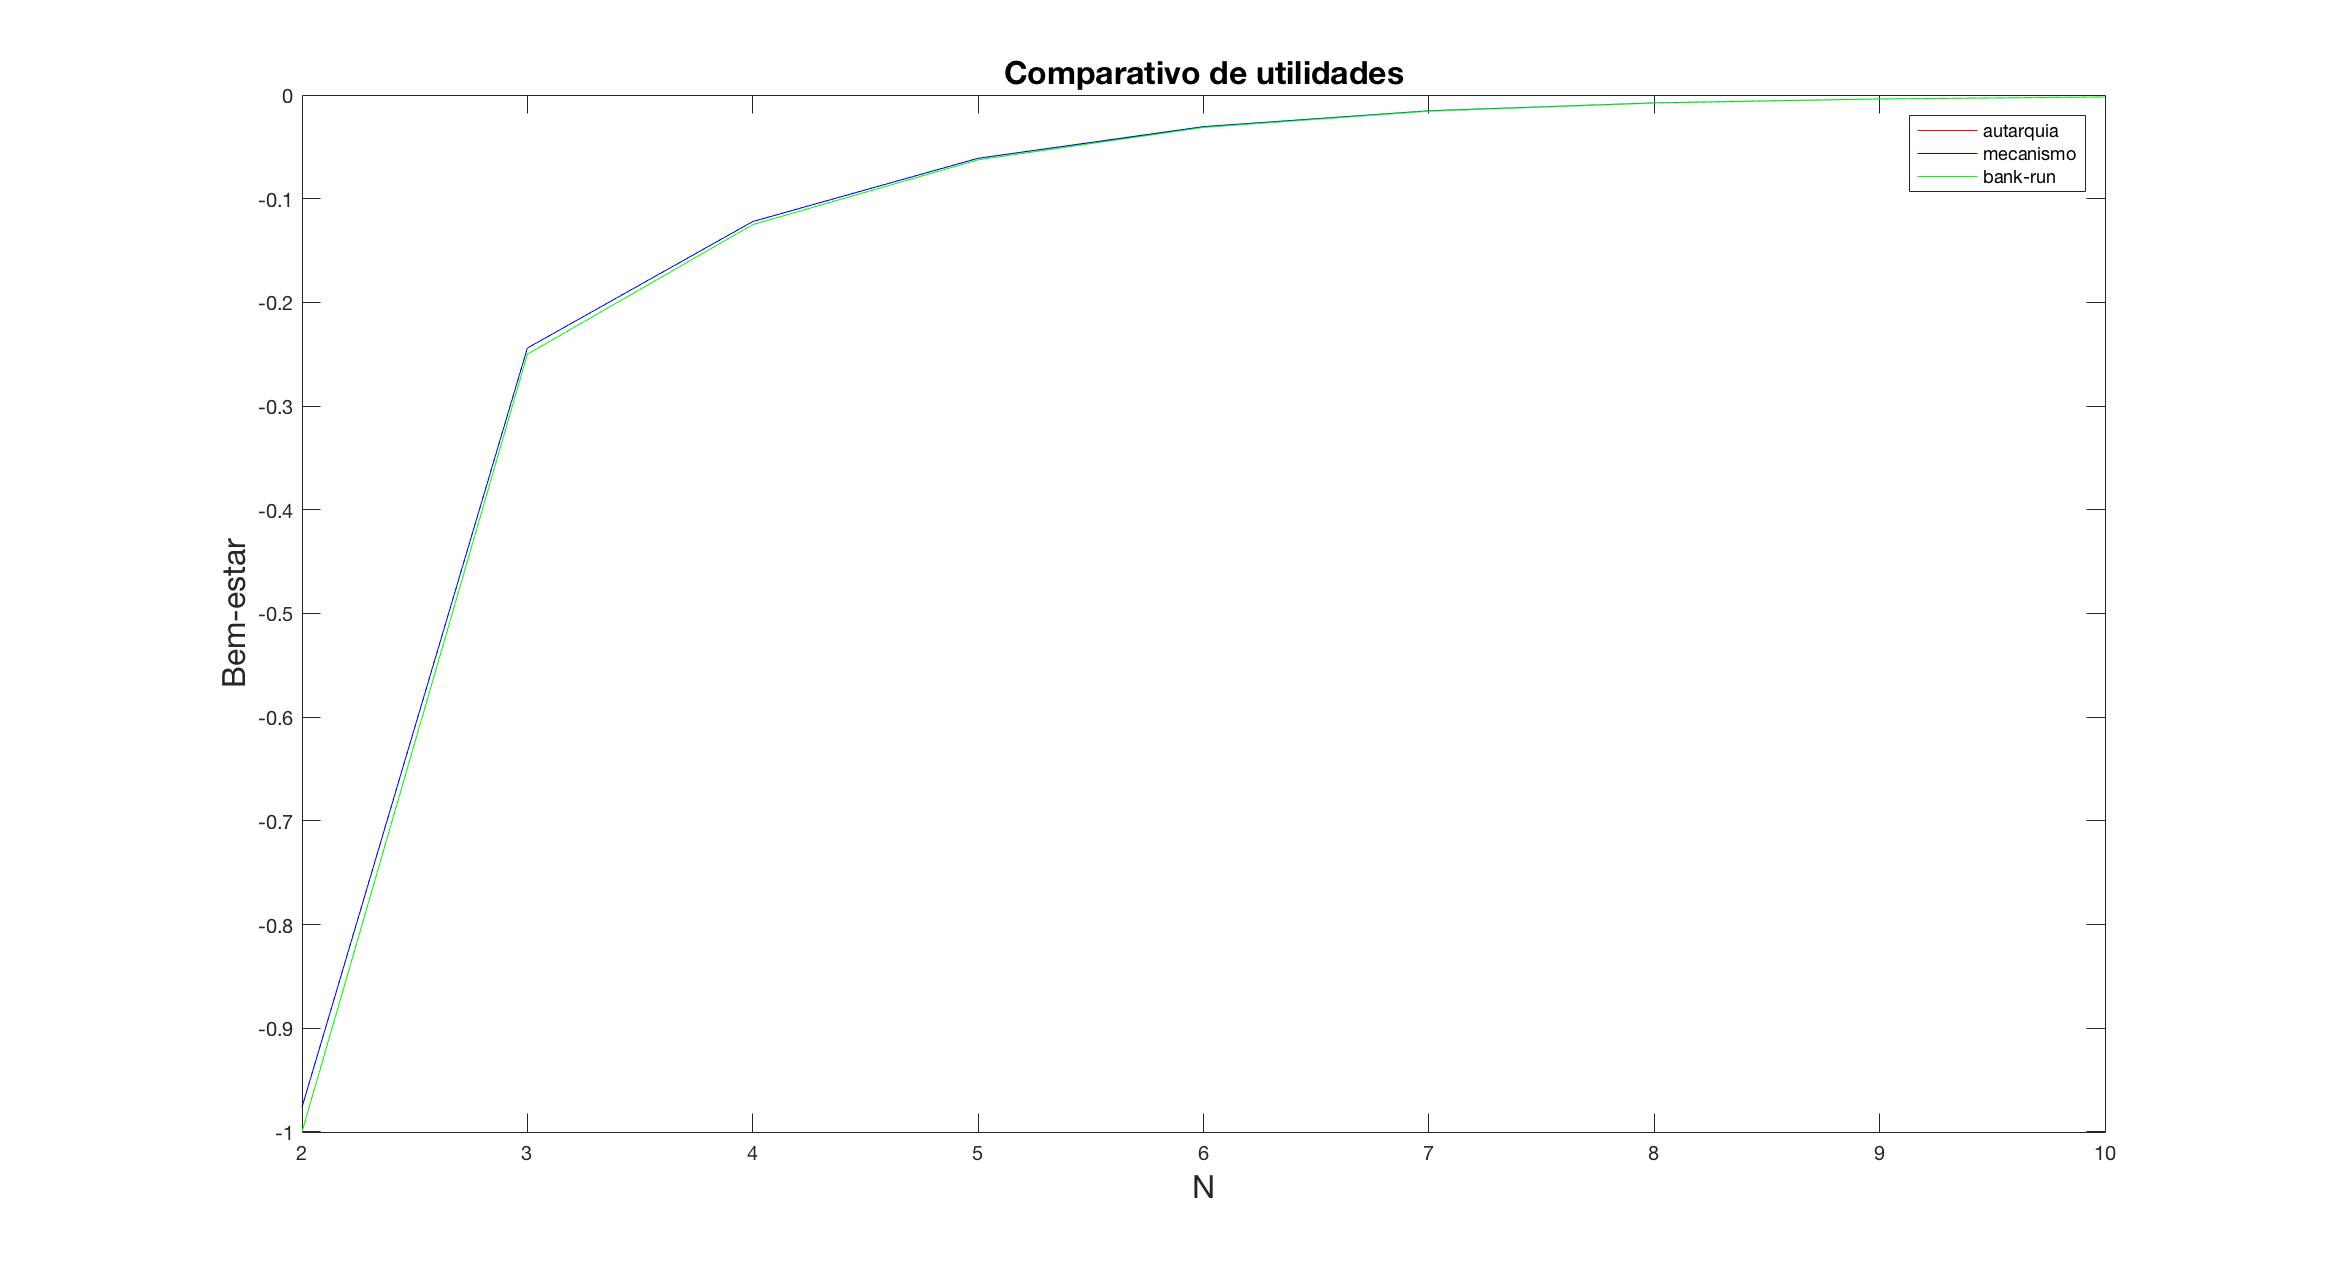
\includegraphics[scale = 0.2]{comparativo}
\end{center}


\section*{Exercício 2}

A simulação numérica realizada (arquivos em anexo) demonstrou que os indivíduos, com o primeiro conjunto de parâmetros utilizados, não têm incentivos a mentirem, ainda que os outros estejam mentindo. Isto caracteriza a possibilidade de implementação do mecanismo direto revelador em estratégias dominantes, de fato. 

Contudo, isto não se sustenta quando o valor do parâmetro A aumenta muito ou mesmo quando N cresce. Nesses casos, há incentivos para não revelar o tipo corretamente, implicando que as truth-telling constraints não estão mais satisfeitas.
\end{document}